\documentclass[xelatex,ja=standard,a4paper,14pt,everyparhook=compat]{bxjsarticle}
\usepackage{amsmath, amssymb, amsthm}
\usepackage{enumerate, mleftright, mathtools}
\usepackage{caption, wrapfig}

% \usepackage{fancyhdr}
% \pagestyle{fancy}
% \fancyhead{}
% \renewcommand{\headrulewidth}{0pt}
% \fancyfoot[C]{}
% \fancyfoot[R]{\thepage}


% \usepackage{zxjatype}
% \renewcommand*\familydefault{\sfdefault}
% % なぜか Segoe UI で () が出力できない
% \setmainfont[BoldFont={Segoe UI SemiBold}]{Segoe UI}
% \setsansfont[BoldFont={Segoe UI Bold}]{Segoe UI}
% \setCJKmainfont{Noto Sans CJK JP}
% \setCJKsansfont{Noto Sans CJK JP}
% \usepackage{concmath}


\usepackage{zxjatype}
% なぜか Segoe UI で () が出力できない
% \setmainfont[BoldFont=* Bold, ItalicFont=* Italic, BoldItalicFont=* BoldItalic]{/usr/local/texlive/texmf-local/fonts/truetype/CMUConcrete/CMU Concrete.ttf}
\usepackage{concmath}
\usepackage[OT1]{fontenc}
\setsansfont{CMU Concrete}
\setmainfont{CMU Concrete}
\setCJKmainfont{Noto Sans CJK JP}
\setCJKsansfont{Noto Sans CJK JP}
% \newfontfamily\bfsegoe{CMU Concrete Roman}
% \renewcommand*\bfdefault{\bfsegoe}


\newcommand{\bbC}{\mathbb{C}}
\newcommand{\fS}{\mathfrak{S}}
\DeclareMathOperator*{\inv}{inv}

\newcommand{\paren}[1]{\mleft(#1\mright)}

\theoremstyle{definition}
\newtheorem{theorem}{定理}[subsection]
\newtheorem{example}[theorem]{例}
\newtheorem{proposition}[theorem]{命題}
\renewcommand{\proofname}{\textup{証明}}

\begin{document}

\section{What is Enumerative Combinatorics?}
\setcounter{subsection}{4}
\subsection{Geometric Representations of Permutations}

\subsubsection{Permutation Matrix}

$w \in \fS_n$について,$n \times n$行列$P_w$を \begin{equation*}
    (P_w)_{ij} = \begin{cases*}
        1 & if $w(i) = j$, \\
        0 & otherwise,
    \end{cases*}
\end{equation*}
で定める.この$P_w$を$w$に対応する\textbf{permutation matrix}という.$P_w$を$n \times n$のグリッドとみなすこともある.

\begin{example}
    長さ$3$の部分減少列を持たない順列$w \in \fS_n$の個数を$f(n)$とする.$P_w$を$n \times n$のグリッドとみなし,$1$の代わりにバツ印を書き入れる.

    条件を満たす$w \in \fS_n$について,$P_w$の左上から右下への最短経路を,次の条件を満たすように書き入れる. \begin{itemize}
        \item 経路はすべてのバツ印の上側,
        \item \textlnot の形の曲がり角は,いずれかのバツ印の右上.
    \end{itemize}

    \begin{figure*}[h]
        \centering
        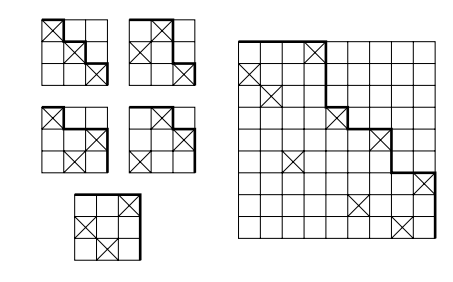
\includegraphics[width=0.6\textwidth]{fig1.4.png}
    \end{figure*}

    \newpage

    こうして得られる経路は対角線より下側を通らない左上から右下への最短経路であり,逆にそのような経路からは,長さ$3$の部分減少列を持たないただ一つの$w \in \fS_n$を対応付けられる(証明略).

    したがって,$f(n)$はカタラン数$C_n = \frac{1}{n+1} \binom{2n}{n}$.
\end{example}

\subsubsection{Diagram}

\begin{wrapfigure}{R}{0.25\textwidth}
    \centering
    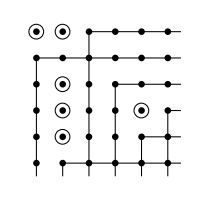
\includegraphics[width=0.25\textwidth]{fig1.5.png}
\end{wrapfigure}

$w \in \fS_n$とする.グリッドを$[n] \times [n]$で表し,各点$(i, w(i))$から右への横線と下への縦線を引く.残った点の集合を$w$の\textbf{diagram}といい,$D_w$で表す.例えば \begin{equation*}
    D_{314652} = \{(1,1), (1,2), (3,2), (4,2), (4,5), (5,2)\}.
\end{equation*}

$j$列目にある$D_w$の要素数を$a_j$とすると,$a_j$は$w$上の値$j$より前に位置する,$j$より大きい要素の個数である.すなわち \begin{equation*}
    I(w) = (a_1, a_2, \ldots, a_n).
\end{equation*}

$i$行目にある$D_w$の要素数を$c_i$とすると,$c_i$は$w$上で位置$i$より後ろに位置する,位置$i$の値より小さい要素の個数である.すなわち \begin{equation*}
    \operatorname{code}(c_1, c_2, \ldots, c_n).
\end{equation*}

また,$D_w^\top = D_{w^{-1}}$(お気持ち記法)が成り立つ.

\begin{example}
    \textbf{$132$-avoiding}な順列を考える.$132$-avoidingでない例:$2143$,$3142$.「長さ$3$の部分減少列を持たない順列」は$321$-avoidingと表せる.

    $w$が$132$-avoidingであることは,$D_w$の点が「左寄せ」になっていることと同値であることが分かる.数列$\lambda_1 \geq \cdots \geq \lambda_n \geq 0$が$\lambda_i \leq n-i$を満たすとき, \begin{equation*}
        D_w = \{(i, j) : 1 \leq j \leq \lambda_i\},
    \end{equation*}
    とすると対応する$w \in \fS_n$が一意に定まる.このような数列$\lambda_1, \ldots, \lambda_n$の個数はカタラン数$C_n = \frac{1}{n+1} \binom{2n}{n}$.

    以上のことから,全ての$u \in \fS_3$について,$u$-avoidingな順列$w \in \fS_n$の個数は$C_n$.
\end{example}

$\#D_w = \inv(w)$より,次が成り立つ.

\begin{proposition}
    $132$-avoidingな$w \in \fS_n$の集合を$\mathcal{S}_{132}(n)$で表すとき, \begin{equation*}
        \sum_{w \in \mathcal{S}_{132}(n)} q^{\inv(w)} = \sum_{\lambda} q^{|\lambda|},
    \end{equation*}
    が成り立つ.ただし$\lambda$は$\lambda_i \leq n-i$を満たす数列$\lambda_1 \geq \cdots \geq \lambda_n \geq 0$を動くとし,$|\lambda| = \sum \lambda_i$とする.
\end{proposition}

\subsubsection{Increasing Binary Tree}

根からのパスが単調増加列になるような,$V(T)=\{1, \ldots, n\}$の根付き二分木を$n$頂点の\textbf{increasing binary tree}という.

$T(w)$を$w$のCartesian treeとするとき,写像$w \mapsto T(w)$は$\fS_n$から$n$頂点のincreasing binary tree全体への全単射である.

\begin{wrapfigure}{R}{0.3\textwidth}
    \centering
    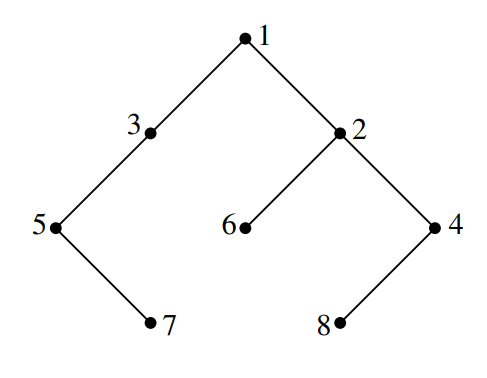
\includegraphics[width=0.3\textwidth]{fig1.8.png}
    \captionsetup{labelformat=empty}
    \caption{例:$T(57316284)$}
\end{wrapfigure}

$w = w_1 w_2 \cdots w_n \in \fS_n$に対して,$w_i$を \begin{itemize}
    \item $w_{i-1} < w_i < w_{i+1}$のとき\textbf{double rise}または\textbf{double ascent},
    \item $w_{i-1} > w_i > w_{i+1}$のとき\textbf{double fall}または\textbf{double descent},
    \item $w_{i-1} < w_i > w_{i+1}$のとき\textbf{peak},
    \item $w_{i-1} > w_i < w_{i+1}$のとき\textbf{valley},
\end{itemize}
と呼ぶ.ただし$w_0 = w_{n+1} = 0$としておく.$w_i$の性質と$T(w)$の頂点$w_i$は,次の対応関係にある.

\begin{table}
    \centering
    \begin{tabular}{r | c}
        $w_i$       & $T(w)$の頂点$w_i$の子 \\
        \hline
        double rise & 右                    \\
        double fall & 左                    \\
        valley      & 左と右                \\
        peak        & なし                  \\
    \end{tabular}
\end{table}

\begin{proposition}
    \begin{enumerate}[(a)]
        \item $n$頂点のincreasing binary treeの個数は$n!$.
        \item ちょうど$k$個の頂点が左の子(または左の子と右の子)を持つようなicnreasing binary treeの個数はオイラリアン数$A(n, k+1)$.
        \item $2n+1$頂点のincreasing binary treeであって,completeであるものの個数は,alternatingな順列$w \in \fS_{2n+1}$の個数と等しい.ここで,complete binary treeとは全ての頂点が$0$個または$2$個の子を持つものである.
    \end{enumerate}
\end{proposition}

※ $A(n, k+1) = \#\{w \in \fS_n : \#D(w) = k\}$.

※ $w$がalternating $\Longleftrightarrow$ $w_1 > w_2 < w_3 > \cdots$.

\begin{proof}
    \begin{enumerate}[(a)]
        \item $\fS_n$からの全単射が存在.
        \item \begin{align*}
                  \text{$T(w)$の頂点$w_i$が左の子を持つ}
                   & \Longleftrightarrow \text{$w_i$がdouble fallまたはvalley} \\
                   & \Longleftrightarrow i-1 \in D(w).
              \end{align*}
        \item \begin{align*}
                  \text{$T(w)$がcomplete}
                  & \Longleftrightarrow \text{$w_1,\ldots,w_n$がいずれもvalleyまたはpeak} \\
                  & \Longleftrightarrow \text{($0 =$) $w_0 < w_1 > w_2 < \cdots$}.
              \end{align*}
    \end{enumerate}
\end{proof}

\subsubsection{Unordered Increasing Tree}

\begin{wrapfigure}{R}{0.3\textwidth}
    \centering
    \includegraphics[width=0.3\textwidth]{fig1.9.png}
    \captionsetup{labelformat=empty}
    \caption{例:$T'(57316284)$}
\end{wrapfigure}

根からのパスが単調増加列になるような根付き木(子の順番は区別しない)を\textbf{unordered increasing tree}という.

$w \in \fS_n$に対して,$0$を根とする根付き木$T'(w)$を次のように構成する.
\begin{itemize}
    \item $1 \leq i \leq n$について,$w$上で値$i$より左に位置する$i$未満で最右の要素を$i$の親とする.そのような要素が存在しなければ,$0$を親とする.
\end{itemize}

このとき,写像$w \mapsto T'(w)$は$\fS_n$から$n+1$頂点のunordered increasing tree全体への全単射である.

\begin{proposition}
    \begin{enumerate}[(a)]
        \item $n+1$頂点のunordered increasing treeの個数は$n!$.
        \item 根が$k$個の子を持つunordered increasing treeの個数は符号なしスターリング数$c(n, k)$.
        \item $k$個の葉を持つunordered increasing treeの個数はオイラリアン数$A(n, k)$.
    \end{enumerate}
\end{proposition}

※ $c(n, k) = \# \{w \in \fS_n : \text{$k$個のサイクルを持つ}\}$.

\begin{proof}
    \begin{enumerate}[(a)]
        \item $\fS_n$からの全単射が存在.
        \item \begin{align*}
            & \#\{w \in \fS_n : \text{$T'(w)$の根が$k$個の子を持つ}\} \\
            ={}& \# \{w \in \fS_n : \text{$k$個のleft-to-right minimaを持つ}\} \\
            ={}& \# \{w \in \fS_n : \text{$\widehat w$が$k$個のleft-to-right maximaを持つ}\} \\
            ={}& \# \{w \in \fS_n : \text{$k$個のサイクルを持つ}\}.
        \end{align*}
        \item \begin{equation*}
            \text{$w_i$が$T'(w)$の葉} \Longleftrightarrow \text{$i \in D(w)$または$i=n$}.
        \end{equation*}
    \end{enumerate}
\end{proof}

\end{document}
